\newpage
\section{Einleitung}
Die Firma MCC Laboratoire Meiners GmbH ist in der Herstellung von Mikroverkapselungen tätig. Neben der Pharma- und Kosmetikbranche werden Mikroverkapselungen auch in der Landwirtschaft eingesetzt. Für diese Branche entwickelt MCC Laboratoire Meiners GmbH Kapseln, sogenannte NemaCaps, welche in der biologischen Schädlingsbekämpfung eingesetzt werden. Ein NemaCap beinhaltet mehrere tausend Fadenwürmer (Nematoden). Der Kapsel ist ein Schlafmittel beigemischt, sodass die Fadenwürmer schlafend gestellt sind. 
\begin{figure}[H]
	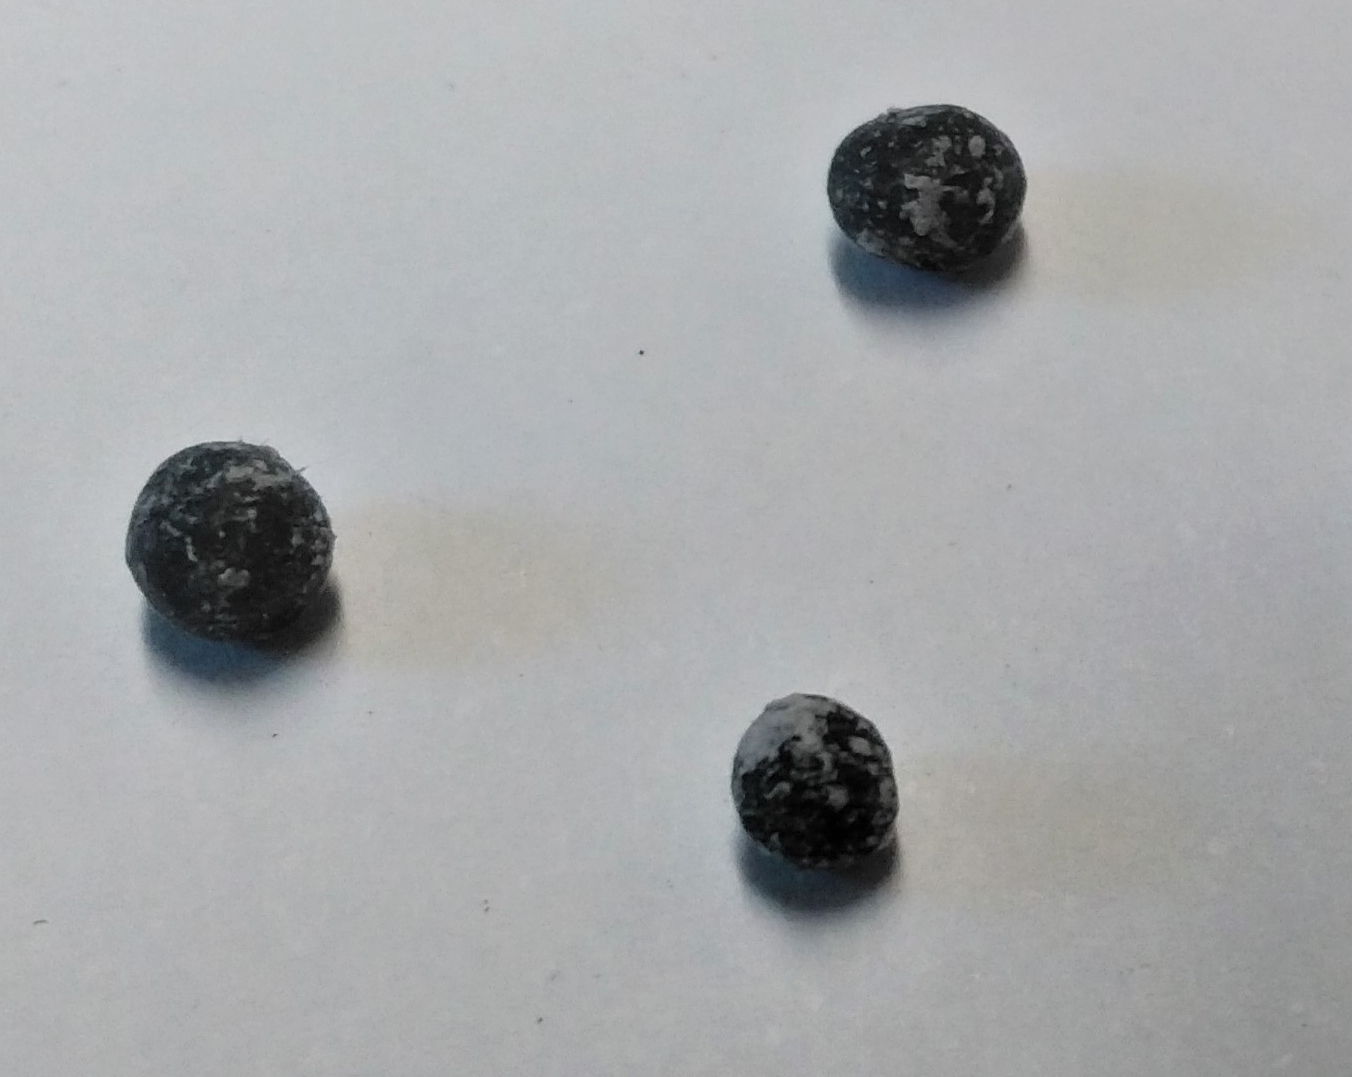
\includegraphics[width=1\textwidth]{Illustrationen/3-Einleitung/nemacaps.jpg}
	\caption{NemaCaps}
	\label{fig:nemacaps}
\end{figure}
NemaCaps werden im Erdreich eingesetzt. Im Wurzelbereich der zu schützenden Pflanze werden diese platziert. Durch das Begiessen der Pflanze oder Regenfall wird das Schlafmittel verdünnt und die Nematoden werden aktiv. Die Hülle der Kapseln besteht aus \textbf{\textit{XYZ}} welches elastische Eigenschaften besitzt. Dies ist Voraussetzung, dass die Nematoden nach dem Aufwachen die Kapsel durchbrechen können.\newline
In ihrer natürlichen Umgebung angelangt stossen die Fadenwürmer nun zufällig auf Larven von Schädlingen. Gemäss dem Nationalen Forschungsprogramm 68 [nachfolgend NFP 68] (2015) dringen die Nematoden durch die Körperöffnungen der Larven ein (Siehe Abb.  \ref{fig:zyklus_Nematoden}, Punkt 3). im Körper der Larve angelangt, setzen die Fadenwürmer dort Bakterien frei (Punkt 1 in Abb.  \ref{fig:zyklus_Nematoden}). Durch die rapide Vermehrung dieser Mikroben wird die Larve abgetötet. Nach Leillinger und Löckener (2012) vermehren sich die Nematoden im Innern der Larve bis diese komplett aufgezehrt ist. Nun verlassen die Nematoden den Kadaver und befallen weitere Larven. So beginnt der Kreislauf erneut von vorne (Punkt 2 in Abb.  \ref{fig:zyklus_Nematoden}).\newline
\begin{figure}[H]
	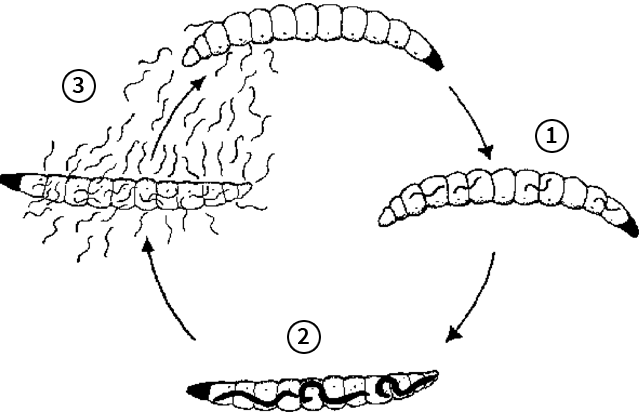
\includegraphics[width=1\textwidth]{Illustrationen/3-Einleitung/zyklus_nematoden.png}
	\caption{Bekämpfung einer Larve durch Nematoden}
	\label{fig:zyklus_Nematoden}
\end{figure}
	
Nach dem NFP 68 (2015) bieten Nematoden speziell in der Bekämpfung gegen Wurzelschädlinge eine wirksame und sichere Alternative zu Pestiziden an, welche im Wurzelbereich weniger gezielt eingesetzt werden können. Dadurch werden die Vorteile der NemaCaps gegenüber von Pestiziden deutlich. Nematoden können im Wurzelbereich gezielt platziert sowie dosiert werden. Ein Vorteil der Kapselung ist die verbesserte Handhabung. Die einfache Lagerung sowie Transport von Fadenwürmer wird möglich.  Zusätzlich wird durch die Verwendung des Schlafmittels die Haltbarkeit der Nematoden verlängert. Diese Vorteile unterstreichen das Potential von NemaCaps, der biologischen Alternative von Pestiziden.

\subsection{Ausgangslage}
Der Einsatz von Nematoden ist im Gartenbau verbreitet. Konventionell werden Nematoden gemäss Birchmeier (\textbf{\textit{2017}}) in Wasser aufgelöst und durch ein Dosiergerät oder eine Spritzkanne in Pflanzennähe aufgetragen. Solche Produkte werden jedoch erst bei erhöhtem Befall von Schädlingen eingesetzt. Der Ansatz der Firma MCC Laboratoire Meiners GmbH ist jedoch ein Anderer. Präventiv möchten Sie Nematoden in Topfpflanzen einsetzen. Im Detailhandel sollen so Topfpflanzen - bereits bestückt mit NemaCaps - im Verkauf angeboten werden.
\newline
Die industrielle Anwendung von NemaCaps birgt bei manueller Bestückung von Töpfen einen hohen personellen Aufwand. 